\documentclass{article}
\usepackage[utf8]{inputenc}
\usepackage{datetime}
\usepackage{enumerate}
\usepackage{textcomp}
\usepackage{amsmath}
\usepackage{amssymb}
\usepackage{tikz}
\usetikzlibrary{arrows,shapes,backgrounds}
\usepackage[edges]{forest}
\usepackage{tikz}
\usetikzlibrary{arrows}

\usepackage{titlesec}
\newcommand{\sectionbreak}{\clearpage}

\title{\bf \Large ASSIGNMENT 5}
\author{Xinhao Luo} 
\date{\today}

\def\math#1{$#1$}

\setlength{\textheight}{8.5in}
\setlength{\textwidth}{6.5in}
\setlength{\oddsidemargin}{0in}
\setlength{\evensidemargin}{0in}
\voffset0.0in

\begin{document}
\maketitle
\medskip

\section{Problem 10.10}
\begin{enumerate}[i)]
    \item \begin{equation}
            \begin{split}
                & gcd(356250895, 802137245) \\
                &= gcd(89635455, 356250895) \Rightarrow 89635455 = 802137245 - 2 \times 356250895 \\
                &= gcd(87344530, 89635455) \Rightarrow 87344530 = 356250895 - 3 \times 89635455 = (-3) \times 802137245 + 7 \times 356250895\\
                &= gcd(2290925, 87344530) \Rightarrow  2290925 = 89635455 - 1 \times 87344530 = 4 \times 802137245 + (-9) \times 356250895\\
                &= gcd(289380, 2290925) \Rightarrow  289380 = 87344530 - 38 \times 2290925 = (-155) \times 802137245 + 349 \times 356250895 \\
                &= gcd(265265, 289380) \Rightarrow 265265 = 2290925 - 7 \times 289380 = 1089 \times 802137245 + (-2452) \times 356250895\\
                &= gcd(24115, 265265) \Rightarrow 24115 = 289380 - 1 \times 265265 = (-1244) \times 802137245 + (2801) \times 356250895\\
                &= gcd(0, 24115) \\
                &= 24115
            \end{split}
    \end{equation}
    \item 
        \begin{equation}
            \begin{split}
                gcd(356250895, 802137245) = 24115 = (-1244) \times 802137245 + (2801) \times 356250895
            \end{split}
        \end{equation}
\end{enumerate}


\section{Problem 10.27(a)}

\math{gcd(6, 15) = 3}, the multiple of 3 can be measured.

\begin{enumerate}[i)]
    \item It is possible. 
        \begin{enumerate}[(1)]
            \item [volumn] 6, 15
            \item 0, 0
            \item 0, 15 (filled)
            \item 6, 9
            \item 0, 9
            \item 6, 3 (target)
        \end{enumerate}
    \item It is not possible since 4 is not the multiple of 3
    \item It is not possible since 5 is not the multiple of 3
\end{enumerate}

\section{Problem 10.40(c)}
\begin{enumerate}[1)]
    \item Evaluating \math{2^{70} \mod {13}}
        \begin{enumerate}[i)]
            \item \math{2^6 \equiv -1 \pmod {13} \Rightarrow 2^{66} \equiv (-1)^{11} \pmod {13}}
            \item \math{2^4 \equiv 3 \pmod{13}}
            \item \math{2^{66} \times 2^4 \equiv -1^{11} \times 3 \pmod {13} \Rightarrow -3 \pmod {13}}
            \item \math{-3 \pmod {13} = 10}
            \item \math{2^{70} \mod {13} = 10}
        \end{enumerate}
    \item Evaluating \math{3^{70} \mod {13}}
        \begin{enumerate}[i)]
            \item \math{3^3 \equiv 1 \pmod {13} \Rightarrow 3^{69} \equiv (1)^{23} \pmod {13}}
            \item \math{3 \equiv 3 \pmod {13}}
            \item \math{3^{69} \times 3 \equiv (1)^{23} \times 3 \pmod {13}}
            \item \math{3^{70} \mod {13} = 3}
        \end{enumerate}
\end{enumerate}

Since \math{10 + 3 = 13} can be divided by \math{13}, \math{2^{70} + 3^{70}} can be divided by \math{13}

\section{Problem 11.6}
\begin{enumerate}[a)]
    \item This graph cannot be done since \math{5 \times 3 = 15} is an odd number.
    \item This graph cannot be done since the maximum degree equals to the total number of the vertices.
    \item This graph cannot be done. The sum of the degree = \math{4 \times 2 = 8}, while the degree listed \math{1 + 2 + 3 + 4 = 10}. 
    \item This graph cannot be done. There are two degrees reach the maximum (\# of vertices - 1), which means that there are two nodes which have connections to all the other nodes. However, there is also a minimum degree 1 which could never be satisfied.
\end{enumerate}

\section{Problem 11.40}

\begin{enumerate}[a)]
    \item No, since there are odd number of domino of each number in the set, while if we want to build a circle, each number should appear even times.
    \item \math{[0,...,n] = (n + 1)+ n + (n - 1) + .... + 1 = \frac{n(n+1)}{2} + (n + 1) = \frac{(n+2)(n+1)}{2}}
    \item Here, we can treat the numbers in the set as vertices. From the constructions, we know that every node has links to the rest of the node.  \\\\
        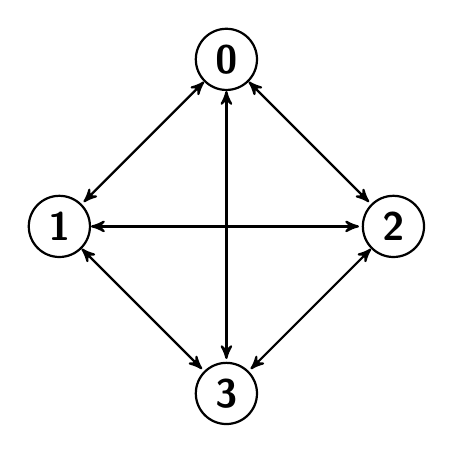
\begin{tikzpicture}[<->,>=stealth',shorten >=1pt,auto,node distance=3cm,
                        thick,main node/.style={circle,draw,font=\sffamily\Large\bfseries}]
    
          \node[main node] (1) {0};
          \node[main node] (2) [below left of=1] {1};
          \node[main node] (3) [below right of=1] {2};
          \node[main node] (4) [below right of=2] {3};
        
          \path[every node/.style={font=\sffamily\small}]
           (1) edge node [left] {} (4)
           (2) edge node [right] {} (4)
           (3) edge node [right] {} (4)
           (1) edge node [left] {} (3)
           (2) edge node [left] {} (3)
           (1) edge node [left] {} (2);
       \end{tikzpicture}
    \begin{enumerate}
        \item  We treat the edge as a domino: for example, an edge between 0 and 1 means card \text{0|1}.
        \item  However, domino has only one combination of between two same number, which mean if we can find a path that go through each edge without repeating, then we definitely can build a circle with the same set of number. 
        \item The number of degrees of each node here should be only be all even or all odd at the same time since each node needs to a link to another, which is \math{n} here.
        \item Since we prove that if we want to walk across each edge repeating them, each node should have even number of degrees; when \math{n} is an even number, the circle can be formed.
    \end{enumerate}
\end{enumerate}

\section{Problem 12.73(l)}

Label the node with number \math{1..9} clockwise. \\

\begin{tikzpicture}[<->,>=stealth',shorten >=1pt,auto,node distance=3cm,
                thick,main node/.style={circle,draw,font=\sffamily\Large\bfseries}]

  \node[main node] (1) {1};
  \node[main node] (2) [below left of=1] {9};
  \node[main node] (3) [below right of=1] {2};
  \node[main node] (4) [below left of=2] {8};
  \node[main node] (5) [below right of=3] {3};
  \node[main node] (6) [below left of=4] {7};
  \node[main node] (7) [below right of=5] {4};
  \node[main node] (8) [below right of=6] {6};
  \node[main node] (9) [below left of=7] {5};

\end{tikzpicture} \\

\begin{enumerate}
    \item It is possible: \math{4, 2, 1, 7, 8, 3, 6, 5, 9} \\
    If we find a way to go through each node without repeating the node (each person can only appear once), that paths will be the way people set around the table.
    \item It is possible: \math{9, 1, 3, 4, 5, 7, 6, 2, 8} \\
    We can make a compliment of the graph (link between those are enemies), and find the paths that go through each node without repeating the node
\end{enumerate}

\end{document}